\documentclass[12pt]{../notes}

% Command for Questions
%\question{}

% Command for Notes
% \note{}

% Code to create a minipage where you can type in class notes. 
%%\begin{minipage}[l][2cm][c]{\textwidth}
%\begin{comment}

%\end{comment}
%%\end{minipage}


% Begin Document
%==============================================================================
\begin{document}
% Include the Title of the Handout
\ntitle{2.2: Diagnostics and Remedial Measures}

\question{1. What happens if the assumptions regarding residuals are not satisfied?}

\begin{minipage}[l][4cm][c]{\textwidth}
%\begin{comment}
\note{
\begin{itemize}
\item The p-values associated with our model rely on proper assumptions regarding the test statistics' ``sampling distributions''.
\item If the residual assumptions are not satisfied, then the sampling distributions are wrong and the p-values are worthless.
\end{itemize}
}

%\end{comment}
\end{minipage}

\question{2. You are running a Box-Cox transformation and the program returns no values...what happened?}

\begin{minipage}[l][2cm][c]{\textwidth}
%\begin{comment}
\note{Most likely problem: your response variable has negative values. Many of the candidate box-cox transformations, such as the natural log transformation, cannot be computed for negative numbers.}
%\end{comment}
\end{minipage}


\question{3. Why would we ever want to make a transformation on an X-variable?}

\begin{minipage}[l][4cm][c]{\textwidth}
%\begin{comment}
\note{
\begin{itemize}
\item A transformation of the X-variable may help to restore a linear relationship between X and Y. 
\item More in module 3: Outlier values in X can make the estimated line fit the majority of the data poorly (called influential points).
\end{itemize}
}
%\end{comment}
\end{minipage}


\question{4. Why would graphical checks (scatterplots, normal probability-plots, etc.) of assumptions be preferred to numerical checks (BF-test of constant variance, correlation test of normality, etc.) of assumptions?}

\begin{minipage}[l][3cm][c]{\textwidth}
%\begin{comment}
\note{
\begin{itemize}
\item Violations of assumptions occur on a spectrum, numerical tests try to force a binary decision.
\item Numerical tests are good to verify potential violations that you suspect based on graphical checks.
\end{itemize}
}
%\end{comment}
\end{minipage}

\newpage
\question{5. Below are two normal probability plots of residuals for a model. For which (if any) of the plots is it acceptable to assume that the residuals follow a normal distribution?}

\begin{figure}[H]
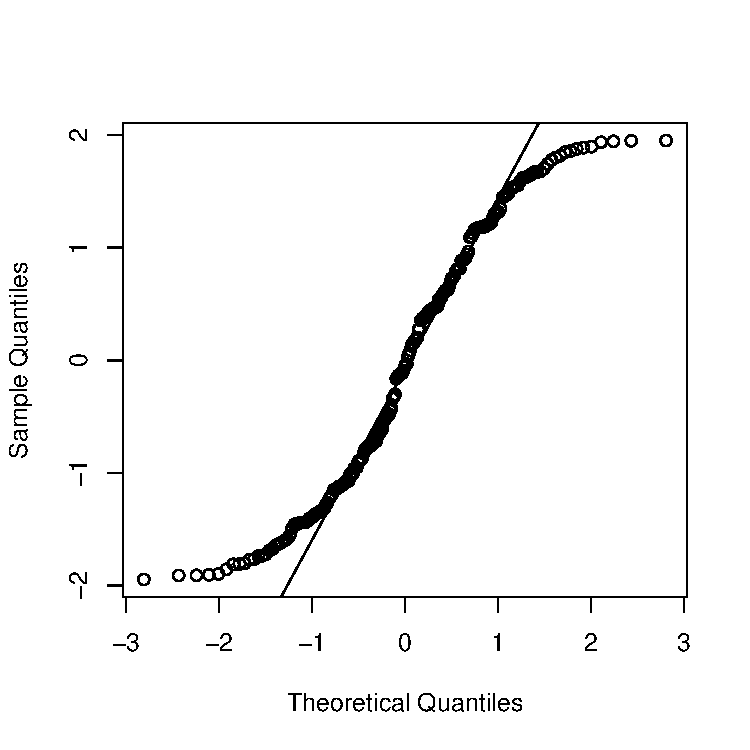
\includegraphics[width = 0.48\textwidth]{../figures/module2/dist_question_short.pdf}
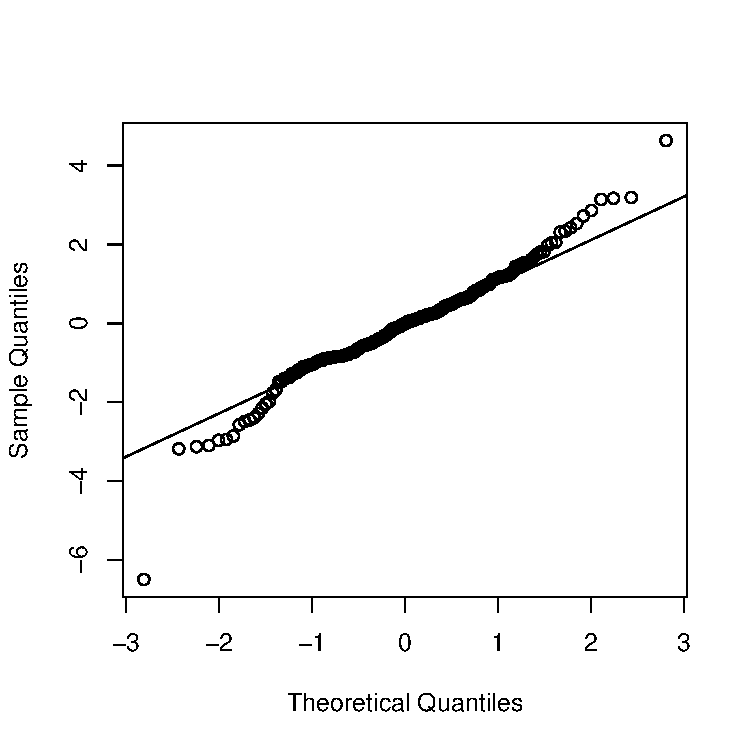
\includegraphics[width = 0.48\textwidth]{../figures/module2/dist_question_long.pdf}
\end{figure}


\begin{minipage}[l][2cm][c]{\textwidth}
%\begin{comment}
\note{It is acceptable to assume that the left plot follows a normal distribution because the tails of this distribution are shorter than what would be expected in a normal distribution. This means that our p-values will be, at worst, slightly conservative (i.e. bigger than they might otherwise be). In general, it is better to over-estimate, rather than under-estimate p-values.}
%\end{comment}
\end{minipage}

\nspace
\question{6. Based on the following output from a Box-Cox Analysis, which transformation would you recommend?}

\begin{figure}[H]
\centering
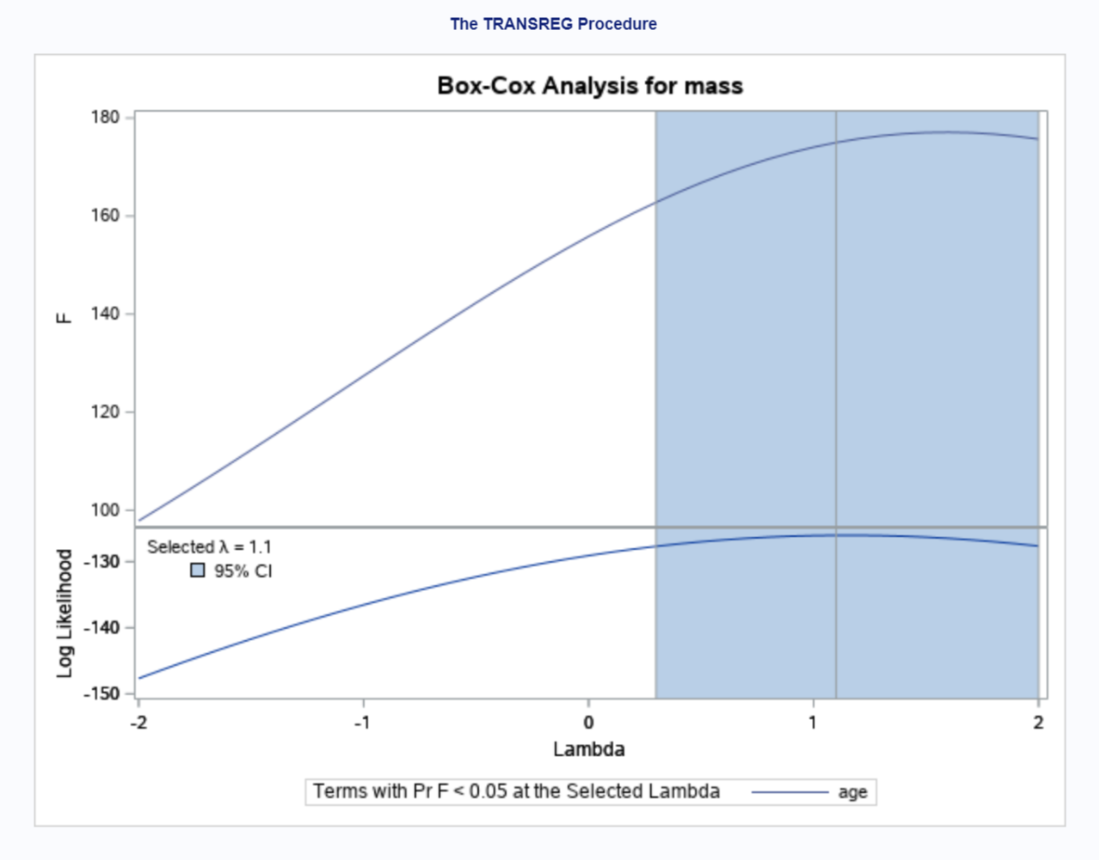
\includegraphics[width = 0.48\textwidth]{../figures/module2/22BoxCox.png}
\end{figure}


\begin{minipage}[l][2cm][c]{\textwidth}
%\begin{comment}
\note{The recommended transformation is close to one. One is well within the confidence bounds of the estimated transformation. Based on this, we would recommend NO transformation.} 
%\end{comment}
\end{minipage}






















% End the Document
%==============================================================================
\end{document}